%\documentclass{sig-alternate-05-2015}
\documentclass[sigconf]{acmart}
\usepackage{url}
%\usepackage{arial}
\let\proof\relax
\let\endproof\relax
\usepackage{amsmath,amsfonts,amssymb,amsthm}
\usepackage{graphicx}
\usepackage{epsfig,multirow, color}
\usepackage{subfigure}
\usepackage{wrapfig}
\usepackage{psfrag}
\usepackage{algorithm}
\usepackage{latexsym}
\usepackage{algorithmic}

\theoremstyle{plain}
\newtheorem{thm}{Theorem}[section]
\newtheorem{lem}[thm]{Lemma}
\newtheorem{prop}[thm]{Proposition}
\newtheorem*{cor}{Corollary}


%\theoremstyle{definition}
\newtheorem{defn}{Definition}
\newtheorem{conj}{Conjecture}
\newtheorem{exmp}{Example}

\theoremstyle{remark}
\newtheorem*{rem}{Remark}
\newtheorem*{note}{Note}

% Code figures
\usepackage{listings}
\definecolor{dkgreen}{rgb}{0,0.6,0}
\definecolor{gray}{rgb}{0.5,0.5,0.5}
\definecolor{mauve}{rgb}{0.58,0,0.82}
\lstset{frame=none,
  language=Java,
  aboveskip=0mm,
  belowskip=0mm,
  showstringspaces=false,
  columns=flexible,
  basicstyle={\tiny\ttfamily},
  %basicstyle={\footnotesize\ttfamily},
  numbers=none,
  numberstyle=\tiny\color{gray},
  keywordstyle=\color{blue},
  commentstyle=\color{dkgreen},
  stringstyle=\color{mauve},
  breaklines=true,
  breakatwhitespace=true,
  tabsize=1
}


%%%%%%%%%%%%%%%%%%%%%%%%%%%%%%%%%%%%%%%%%%%%%%%%%%%%%%%%%
%%%%%%%%%%%%%%%%%%%%%%%%%%%%%%%%%%%%%%%%%%%%%%%%%%%%%%%%%
%  USE THIS? (To move table caption down)
 \usepackage{caption}
 %\captionsetup[table]{skip=5pt}
%%%%%%%%%%%%%%%%%%%%%%%%%%%%%%%%%%%%%%%%%%%%%%%%%%%%%%%%%%
%%%%%%%%%%%%%%%%%%%%%%%%%%%%%%%%%%%%%%%%%%%%%%%%%%%%%%%%%%


\usepackage{booktabs} % For formal tables
%\setcopyright{none}

\begin{document}

\title{Hardware Isolation Mechanisms for Security Improvement in FPGAs}
%
%\author{Festus Hategekimana}
%\affiliation{%
%  \institution{University of Arkansas}
%  \city{Fayetteville}
%  \state{AR}
%  \country{USA}}
%  \email{fhategek@uark.edu}
%
%\author{Taylor JL Whitaker}
%\affiliation{%
%  \institution{University of Arkansas}
%  \city{Fayetteville}
%  \state{AR}
%  \country{USA}}
%  \email{txw043@uark.edu}
%
%\author{Md Jubaer Hossain Pantho}
%\affiliation{%
%  \institution{University of Arkansas}
%  \city{Fayetteville}
%  \state{AR}
%  \country{USA}}
%  \email{mpantho@uark.edu}
%
%\author{Christophe Bobda}
%\affiliation{%
%  \institution{University of Arkansas}
%  \city{Fayetteville}
%  \state{AR}
%  \country{USA}}
%  \email{cbobda@uark.edu}


\begin{abstract}
Field Programmable Gate Arrays (FPGAs) platform security management continues to be a strong area of concern despite recent increased adoption and integration of FPGAs into commercial scale cloud computing systems. One of the technical problems in the FPGA security management area has been the lack of hardware primitives to support multi-tenancy while enforcing proper domain isolation. In this tutorial, we present recent progress that has been made to address this issue. Specifically, we present hardware isolation mechanisms that can be used to enable domain separation on FPGA based systems. We demonstrate the viability of these mechanisms through a software-hardware codesign implementing a simple TSL/SSL encryption application.
\end{abstract}


\begin{CCSXML}
<ccs2012>
<concept>
<concept_id>10002978.10003001.10003003</concept_id>
<concept_desc>Security and privacy~Embedded systems security</concept_desc>
<concept_significance>500</concept_significance>
</concept>
<concept>
<concept_id>10002978.10003001.10003599</concept_id>
<concept_desc>Security and privacy~Hardware security implementation</concept_desc>
<concept_significance>500</concept_significance>
</concept>
<concept>
<concept_id>10010583.10010600.10010628.10011716</concept_id>
<concept_desc>Hardware~Reconfigurable logic applications</concept_desc>
<concept_significance>500</concept_significance>
</concept>
</ccs2012>
\end{CCSXML}

\ccsdesc[500]{Security and privacy~Embedded Systems Security}
\ccsdesc[500]{Security and privacy~Hardware Security Implementation}
\ccsdesc[500]{Hardware~Reconfigurable Logic Applications}
\keywords{FPGA Security, Hardware Isolation, IP Containerization, CAPSL}


\maketitle


\section{INTRODUCTION}\label{sec:intro}
Many of today's critical embedded systems are increasingly relying on FPGA-based SoCs because of the useful balance between the performance, scale, flexibility, and rapid time to market they provide. This was recently exemplified with the recent Audi announcement that its 2018 A8 world's first Level 3 autonomous driving system will feature Altera's Cyclone FPGA SoCs for object and map fusion processing tasks. Though, it's not just in embedded systems space where we are seeing accelerated adoption of FPGA platforms, as they are also being continuously integrated into commercial scale cloud computing systems and data centers as evidenced by Amazon recent announcement of providing cloud compute instances with FPGAs (EC2 F1).

This increased adoption of FPGA into commercial scale cloud computing systems has highlighted the issue of FPGA's lack of hardware primitives, conceptually similar from a security perspective to a CPU's IO memory management unit (IOMMU), to support multi-tenancy while enforcing proper domain separation among the tenants (i.e. multiple applications utilizing the same FPGA) \cite{CloudFPGA}, \cite{CapslHOST}, \cite{Byma2014FPGAsIT}. This lack of native support for isolation creates security concerns where: 1) Since FPGA accelerators tend to run with full hardware access, a single accelerator vulnerabilities can be exploited through traditional system software stacks or if malicious, can bring down a shared compute host \cite{CloudFPGA}. Or 2) tenants are not able to protect confidentiality and integrity of their application  data not only from other tenants, but also from other unauthorized parties including privileged system software, such as the hypervisor \cite{sconee}.

An effective solution to the problem of lack of proper domain separation on FPGAs should be able to enable scaling of security across a range of system parameters, such as power and performance, without significant drop in coverage. We believe and intend to demonstrate in this tutorial that this can only be achieved through some form of combination of measures that protect against hardware vulnerabilities directly at the hardware level and measures that enforce domain separation at the software level.In this tutorial, we look at a set of  research works that individually attempted to address the problem of lack of isolation support on FPGAs. We demonstrate how certain elements of these works can be put together to provide an effective and comprehensive solution to this problem. We demonstrate the viability of this solution through a real-world software-hardware codesign application which implements a simple TSL/SSL encryption.

The remainder of this work is organized as follow: Section \ref{sec:threat_model} starts by describing the specific use case scenarios and security concerns this method addresses. Section \ref{sec:problem_definition} gives an overview of research works that form the basis of our comprehensive solution. Section \ref{sec:application} and Section \ref{sec:Implementation} conclude the paper with a tutorial demonstrating how a combination of the discussed approaches can be used to provide proper domain isolation on FPGA platform.

\begin{figure}[h]
\centering
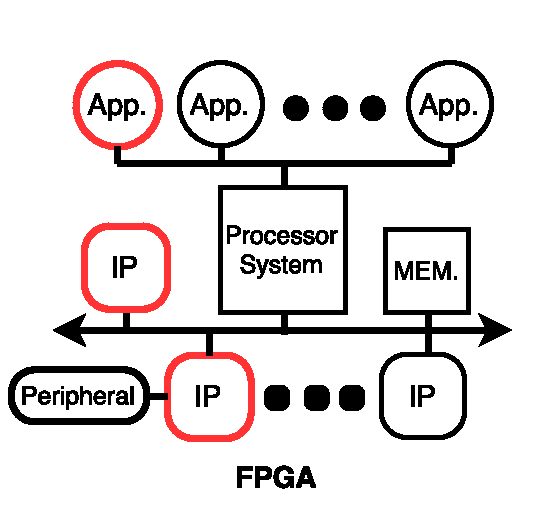
\includegraphics[width=0.5\columnwidth]{figures/ThreatModel.pdf}
\caption{Embedded system threat model: The adversary controls the FPGA SoC and can execute malicious code (non-trusted application + accelerator in red) remotely and launch a denial-of-service attack to an IO component.}
\label{fig:threat}
\end{figure}

\section{THREAT MODEL} \label{sec:threat_model}

This section describes the threat model for two use case scenarios our approach targets. We first look at the attack surface in FPGA-based embedded systems and then, we look at FPGA security concerns in cloud computing systems integrating FPGAs.

\subsection{Embedded Systems}

The illustration of our threat model in Figure \ref{fig:threat} shows the first use case scenario our approach targets. We assume an adversary who can introduce hardware trojans in the IPs during development (supply chain attack). We assume this adversary will later have a remote access to the FPGA system-on-chip (FPGA SoC) which contains some of the malicious IPs. We assume the adversary is aware of the trojans activation mechanisms and can only activate them externally by executing some malicious input for example.

In FPGA-based SoCs, we do not current have hardware-level support mechanism that would prevent unauthorized bus data access by a bus component. We rely on bus protocols which generally assume that bus components are going to adhere to the protocol and wait for their turn to broadcast. However, this is not always the case since a malicious component can unilaterally decide to access the bus and launch a denial-of-service (DoS) attack for example to a system peripheral.



\subsection{FPGAs in the Cloud}

The fast adoption of FPGA accelerators in cloud computing and the probable future adoption in personal computers raise additional security concerns. Cloud providers such as Amazon that provide infrastructure as a service, must address security threats posed by malicious IPs residing on FPGA without affecting the performance of the system. In general, security is enforced in cloud computing using domain separation. User are assigned virtual instances (VIs) which are then scheduled on physical resource under by a hypervisor. The hypervisor controls the access to the hardware and insure that every virtual instance remain active within its limit. As shown on Figure \ref{fig:iaas-fpga}a), such an approach requires resource virtualization, for which no viable solution currently exist in FPGA. As a result, whole FPGAs must be assigned to small accelerators thus wasting resource , or the execution on the FPGA must be emulated in the hypervisor with performance degradation.

\begin{figure}[h]
\centering
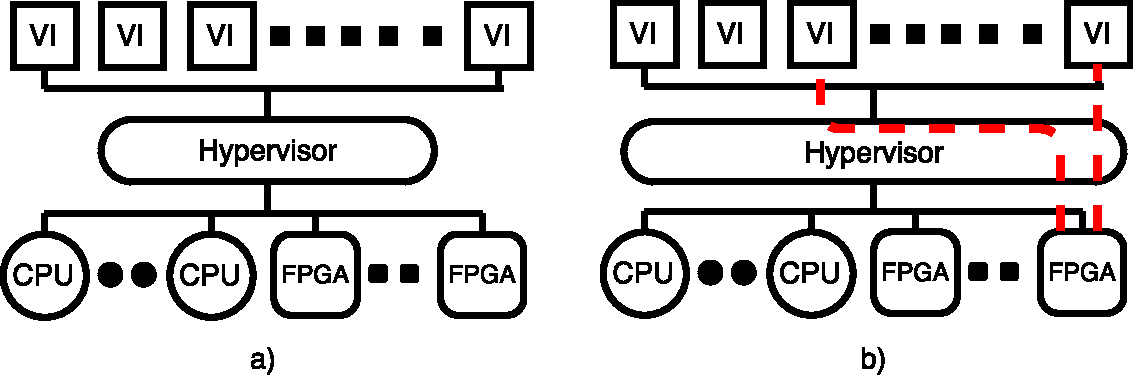
\includegraphics[width=0.45\textwidth]{figures/CloudThreatModel.pdf}
\caption{FPGA provisioning in IAAS-based cloud computers. FPGAs are virtualized in (a) and in (b), tenants are granted direct access to the FPGAs.}
%\vspace{-6pt}
\label{fig:iaas-fpga}
\end{figure}

An optimal use of FPGA resource would allow FPGA to be share among IPs, sometimes from different tenants for a better FPGA utilization without performance degradation. With several IPs on the same FPGA, there is currently no mechanism to guarantee that some IPs will not perform malicious activities, even in the presence of strong protocols. The classic approach to enable IPs on the FPGA is through registers directly controlled by the hypervisor (for the purpose of domain separation), and accessible to the corresponding instance (Figure \ref{fig:iaas-fpga}b). The problem here is that a trojan hidden into an IP can bypass protocol and place data on FPGA lines to cause harm. Since the connections are well known, nothing prevent an IP designer to tap long FPGA lines and read information from neighbor modules or to write on line randomly to DoS the design on the FPGA in cloud. As we will show in this tutorial, hardware isolation can address domain separation in hardware to provide an increase protection in the cloud.

\section{HARDWARE ISOLATION MECHANISMS} \label{sec:problem_definition}

Protection of sensitive data in networked and embedded systems has become a critical problem with far-reaching financial and societal implications. Among the 10 paradigms (Deception, Separation, Diversity,  Consistency, Depth, Discretion, Collection , Correlation, Awareness, Response)  used to address cybersecurity, separation is one of the most effective and relatively easy to implement and, thus increasingly used to address security, in particular in web application where security concerns have been the highest (\cite{Mello2015,  JonesCU, Fireglass2016, Cottrell2017}. The Google Chrome and Adobe have been successfully relying on isolation in the form of sandboxes (\cite{chromiumSB, adobeSB}) to isolate non-trusted code remotely provided to users for execution on their computers. Isolation has proved to be a very effective mechanism and could play a vital role in protection of malicious activities in hardware. The goal of this tutorial is therefore to provide users a tool for a seamless design and deployment of efficient hardware isolation techniques to address security concerns in FPGA-based systems.

The remainder of this section discusses current techniques that are employed to enforce hardware isolation on FPGAs. This list is by no means exhaustive and it is beyond the scope of this paper to discuss these techniques in greater details. The interested reader is encouraged to refer to cited works.

\subsection{Reference Monitors}

In this approach, a hardware module or a microcontroller based firmware-upgradable module is used to monitor and enforce authorized sharing of system
resources among cores. Memory-access security policies are expressed in a specialized language, and a compiler translates these policies directly to a circuit (or a microcontroller) that enforces the policies. The circuit is then loaded onto the FPGA along with other components of the system.

There are many research efforts with some relation to this approach, but to the best of our current knowledge, works in \cite{HuffEmbedded} and in \cite{Huffmire} are the only work with similar goals that come close to ours here. In their work, they designed and implemented a reconfigurable reference monitor (RM) which implements an access control list (ACL). They then integrated the reference monitor into the on-chip peripheral bus (OPB) and used it to regulate access to the memory and peripherals. Memory and peripherals accesses go through a reconfigurable monitor's access control list [3]. The access control list associates every object (memory ranges for ex.) in the system with a list of principals (IP cores) with the rights of each principal to access the object[3]. In their implementation, each object access has to be computed by the reference monitor's ACL at runtime. The decision is either granted access or denied access. Since this access model can create potential memory performance issues in large memory applications, they proposed a mechanism in which a buffer is used to hold the data until the ACL grants approval of the legality of the request \cite{SPHuffmire}. Figure \ref{fig:ted} illustrates the implementation. For example, in case of a write, the data to be written is stored in the buffer until the ACL grants the approval, at which time the write request is sent to the memory \cite{SPHuffmire}.


\begin{figure}[hbt]
\centering
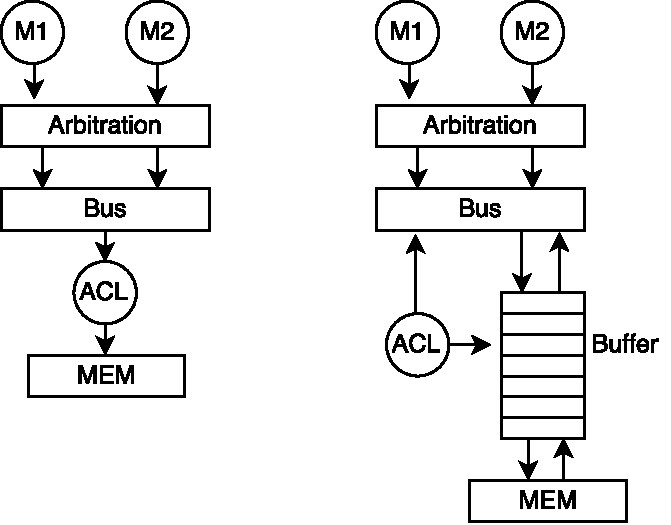
\includegraphics[width=0.75\columnwidth]{figures/ted_access.pdf}
\caption{Access Model Implementation. On the left, there's no "caching" mechanism. On the right, a buffer is used to hold the data while access rights are being looked up.} % The text in the square bracket is the caption for the list of figures while the text in the curly brackets is the figure caption
\label{fig:ted}
\end{figure}



Authors in \cite{FestusFCCM} observed that in Huffmire et al. access model implementation if you had consecutive and repeated memory access from the same ``principal" to the same ``object", each one of these requests would still have to go through the reference monitor's computation. This can potentially create performance issues in large designs. These issues can be avoided by adding the capability to remember access decisions. Authors in \cite{FestusFCCM} built upon this observation and proposed an improved implementation of this architecture by adding capability to remember access decisions to allow them to be administered at run-time without re-computations. Figure ~\ref{fig:access} shows their proposed access model.

\begin{figure}[hbt]
\centering
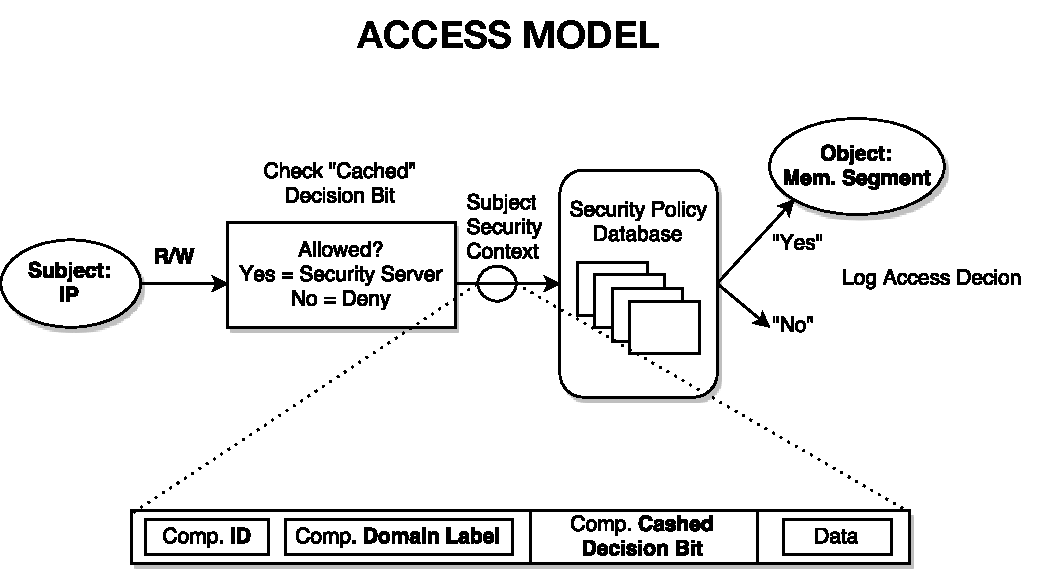
\includegraphics[width=1\columnwidth]{figures/access.pdf}
\caption{Improved Access Model Implementation.} % The text in the square bracket is the caption for the list of figures while the text in the curly brackets is the figure caption
\label{fig:access}
\end{figure}

Both of these techniques follow a similar design flow. Systems components are defined and implemented using hardware synthesis tools such as Xilinx's Vivado or Xilinx's XPS.  The hardware-enforced ACL core is generated by some policy compiler and it's then integrated with the rest of the system components similar to adding a standard custom IP to your design [CITAT],[CITAT]. In some instances, however, there can be compatibility issues. Sometimes standard integration of the ACL core can be complicated with the fact that some security-relevant attributes may not be directly available as parameters or easily derived from available parameters. For example, the current version of the AXI Interconnect IP core API available in Vivado 2016 does not present a component ID as a parameter. In situations like these, it's up to the application designer to build their own custom OPB (or AXI interconnect) IP which directly integrates this ACL security functionality.

Authors in \cite{proofcarrying}, \cite{proof}, \cite{proofcar} observed that the above described techniques assume a ``trusted" reference monitor to enforce the security policies and with no mechanism through which the platform itself can authenticate the authority of the reference monitor before it administers an access policy decision. The security concern here is that an attacker could conduct a man-in-the-middle attack on the system by inserting a malicious circuit inside the only authority entrusted with administrating shared resource access decisions. To mitigate this, they proposed an improved implementation of the reference monitor which combines the monitoring approach with a ``proof-carrying hardware" concept. Their approach consisted of using a consumer-producer approach, where a consumer specifies a desired functionality of the memory access monitor and sends this specification to the producer and the producer synthesizes this information into a bitstream \cite{proofcarrying}. The producer re-extracts the logic function from this bitstream and, together with the original specification, computes some miter function (which outputs an error flag if the specification and implementation differ for at least one input vector) \cite{proof}. This proof of reference monitor correctness is then generated along side with the bitstream and is sent to the consumer. The latter verifies the proof, and in case of success partially reconfigures the monitor with security policies \cite{proof}. The consumer verifies the proof of correctness from the producer by extracting the monitor's logic function from the bitstream and forms a miter in conjunctive normal form in the same way as the producer, but with the original specification. This new miter is compared to the producer's miter and if they both match, the implementation is accepted and the monitor is accepted. The monitor is rejected if the the miters do not match \cite{proof}, \cite{proofcar}.


\subsection{Secure Enclave: Zynq FPGA TrustZone}

In this approach, systems developers rely on an operating system and some hardware-level enforcement mechanisms to provide system security services. Security features provided include, but are not limited to, confidentiality and integrity protection of the external memory containing the sensitive application code and data.

A recent example of this approach is the ARM TrustZone security architecture currently available to Zynq-7000 SoC. The latter supports ARM TrustZone technology in both the PS and PL domain. The ARM TrustZone architecture makes trusted computing within the embedded world possible by establishing a trusted platform, a hardware architecture that extends the security infrastructure throughout the system design. Instead of protecting all assets in a single dedicated hardware block, the TrustZone architecture runs specific subsections of the system either in a ``normal world" or a ``secure world."

In the Zynq-7000 AP SoC, a normal world is defined as a hardware subset consisting of memory regions, L2 cache regions, and specific AXI devices. The Zynq-7000 AP SoC supports ARM TrustZone technology in both the PS and PL domains of the device. The PS provides a set of configuration registers related to TrustZone support for custom IPs. These configuration registers are then dynamically programmed by the software during execution. All slave IP cores instantiated in the logic can be individually assigned a Secure or Non-Secure designation. For Xilinx slave IP cores, Secure/Non-Secure configuration can be statically designated at the AXI interconnect level during system creation process.

Figure \ref{fig:ted} shows a simplified example of how to secure your design sensitive components from illegal hardware access using Zynq-7000 AP SoC TrustZone technology

\begin{figure}[hbt]
\centering
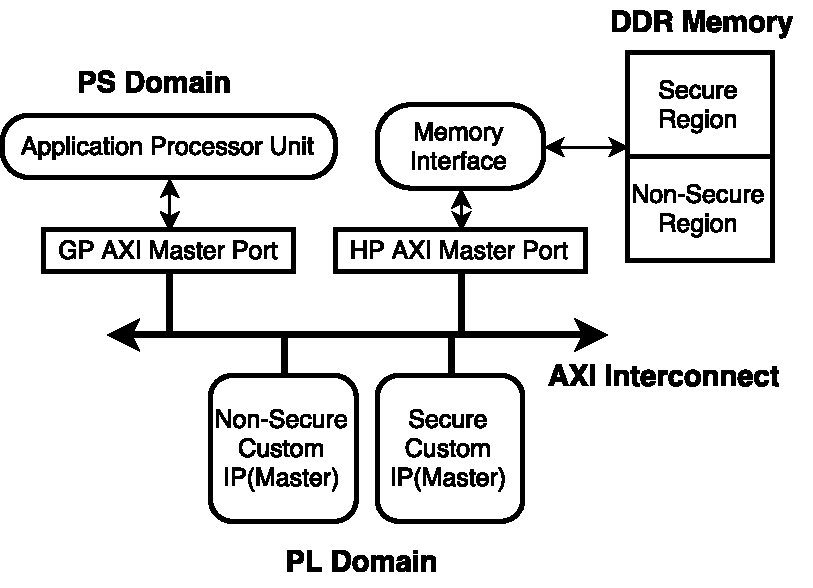
\includegraphics[width=0.75\columnwidth]{figures/TrustZoneHardware.pdf}
\caption{Improved Access Model Implementation.} % The text in the square bracket is the caption for the list of figures while the text in the curly brackets is the figure caption
\label{fig:trustzone}
\end{figure}

In this example, also available in [], on the hardware level the PL domain uses two custom master IP cores:

\begin{itemize}
\item \textbf{Secure Custom IP:}
This performs Secure read/write transactions to DDR using the HP slave port in the PS. It is also connected to the Application Processor Unit (APU) via a GP master port for register configuration.
\item \textbf{Non-Secure Custom IP:}
This is used to perform read/write transactions from/to the PS DDR upon requests from the external world. It performs Non-Secure read transactions to DDR using an HP slave port. Configuration of this IP is done by the PS processor through a GP master port.
\end{itemize}

Upon power-on, the PS processor initializes both custom IPs, configures registers to establish Secure and Non-Secure regions in DDR memory, and transfers private data/instructions to the Secure DDR region. After initialization and upon receiving a data request from the external interface, the
Non-Secure custom IP first copies the data from the external interface to the Non-Secure region of DDR memory. It then interrupts the PS processor, which commands the Secure custom IP to perform the appropriate data computations using its private data/instructions in conjunction with the data just copied to the Non-Secure region of DDR memory. After computation is completed, Secure custom IP puts the computed data into the Non-Secure DDR region and interrupts the PS processor to command the Non-Secure custom IP to start transferring data from the requested location.

On the software level, application processes (and their IPs) with non-secure status designation execute in memory space separated from processes with secure status designation. When a user process running in the Non-Secure world requires Secure execution, it makes a request to the Non-Secure kernel to enable the TrustZone Secure Monitor to transfer execution of the process to the Secure world. The Secure Monitor mode links the two zones and acts as a gatekeeper to manage program flow between them.

To ensure integrity of the TrustZone software, Zynq-7000 provides a secure boot flow; where the on-chip BootROM code starts the whole security chain by ensuring that first-stage bootloader (FSBL) is signed and verified.

\subsection{Hardware Sandboxing}\label{sec:HardwareSandbox}
The approach of utilizing hardware sandboxes for isolating and identifying potential malicious IP-internal circuits provides a flexible design process for systems designers and integrators. Similar to discussed approaches, a sandbox isolates IP by partioning the hardware design to a trusted secure region and a non-trusted environment contained within the sandbox. It supports the following security policies: Isolation policy that limits the IP to only allowable interactions, Containment policy that minimizes the damage caused by a malicious component, and Integrity policy that enforces authorized data accessibility and modifications. These policies are implemented through two distinct but complementary mechanisms: \textit{ Complete Mediation, and  Resources Virtualization}.

Hardware sandboxing allows the placement of interface-level behavioral monitors, collected in a \textit{``Checker"} component that implements the \textit{Complete Mediation} mechanism by checking every interaction made by the user IP to the system and only authorizing allowable interactions as specified by the IP interface specification.

The \textit{``Sandbox controller"} implements the \textit{Resources Virtualization} mechanism by providing both virtual memory buffers (local to the user IP) and virtual IO access for critical resource protection. It also generates a \textit{``virtual resources controller"} in case there are more virtual resources competing for a single physical resource. \textit{``Status registers"} are used to monitor and log the user IP security status. This is useful in that a subverted IP can't launch a denial-of-service attack by repeatedly making illegal requests. Also, this can be used to log the user IP if it triggers a Trojan at run-time for example. This information can then be used to blacklist some vendors from the integrator's list of contractors.




\section{SECURITY CRITICAL EXAMPLE APPLICATION} \label{sec:application}

In this section, we introduce an example application to demonstrate the various hardware isolation methods discussed above.

% We propose a system that performs secure encryption processes (via Hardware-enfored Access Lists and TrustZone) alongside potentially malicious non-secured processes.

% With our secure process utilizing hardware-accelerated encryption, CAPSL is utilized to secure the encryption engine and enforce the integrity of its behavior. This system suits the implementation of the discussed hardware isolation methods with the inclusion of points of attack in both software and hardware.
%
% Below, we detail the example application and address the security vulnerabilites with regard to the introduced isolation methods.


\subsection{Overview}

We intend to demonstrate the steps required to ensure the protection of a general security-critical system design with an SoC system providing reconfigurable fabric along with a co-processor. The discussed isolation methods enforce security at the OS/PS level down to the hardware IP interface level. Thus, our demonstration application includes process level applications running on the processing system while hardware is utilized for acceleration cores. The system requires a security critical application such an application requiring sensitive keys to be handled at the software level while relying on hardware for accelerating cryptographic functions.

\subsubsection{Secure Echo Server Process:}
We utilize an echo server that encrypts client communcations with a session key established through a simplified TLS/SSL handshake. This system setup assumes the server to be run on the SoC device targeted for protection while the client is run on a remote machine. The SoC hosting the echo server is designed to run on a Zynq SoC, with the zynq processor hosting a Linux OS and utilizing FPGA area for cryptographic functions. The echo server process and complementing client process are implemented as Python programs. We used Xilinx's Petalinux tool for generating the design images required to boot a Linux OS and mount the filesystem. We implemented our system on a Digiglent Zybo [IT MIGHT NOT BE BIG ENOUGH for AES + RSA]...

\begin{figure}[]
\centering
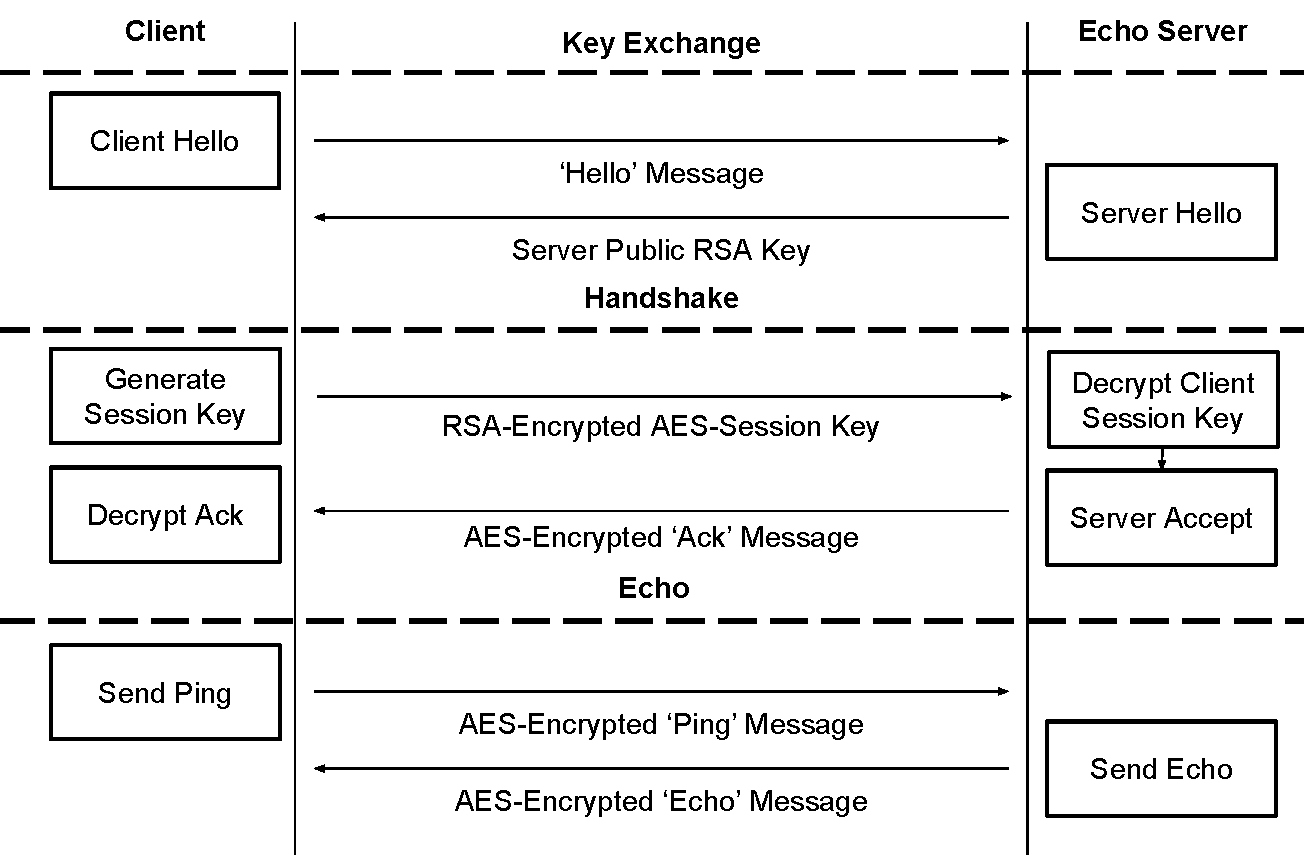
\includegraphics[width=1\columnwidth]{figures/ProcessInteractions.pdf}
\caption{Baseline Behavior for Client and Echo Server}
\textit{In its initial state, the server process listens on a specified network IP address and port awaiting a client connection. Upon receiving a connection, a handshake is initiated as the server immediately shares an RSA public key. A session key computed by the client is received by the server encrypted with its public RSA credentials. Deciphering this session key allows subsequent communications to be secured, namely the server's acknowledgement of a successful handshake, the client's message, and finally the server's echoed message.} % The text in the square bracket is the caption for the list of figures while the text in the curly brackets is the figure caption
\label{fig:ProcessInteractions}
\end{figure}

% To further elaborate on our application, we begin with the echo server process.

% The its initial state, the server process listens on a specified network IP address and port awaiting a client connection. Upon receiving a connection, a handshake is initiated as the server immediately shares an RSA public key. A session key computed by the client is received by the server encrypted with its public RSA credentials. Deciphering this session key allows subsequent communications to be secured, namely the server's acknowledgement of a successful handshake, the client's message, and finally the server's echoed message.
% This system behavior as seen at the process level can be seen in Figure \ref{fig:ProcessInteractions}.

\subsubsection{Hardware Accelerated Encryption Engine:}
The handshake requires the use of both symmetric-key and public-key algorithms, as a symmetric-key (used as session key) is generated from utilizing a asymmetric-key to encrypt and publically transmit the session key. AES and RSA are commonly used to meet these requirements. As these can be computationally expensive with larger key sizes, one standard application of hardware acceleration is for performance boosts with cryptographic functions. To provide our demo system with a hardware component, an AXI-bus enabled IP core is used to accelerate the AES and RSA algorithms used by the echo server process. The PS and PL interaction is detailed in [NEED DIAGRAM].

Upon requiring the AES or RSA cores during execution, data is first written to the appropriate input data registers for each IP. After a successful write of input data, an enable signal is written to a control register to signal the IP core to perform the encryption/decryption. A set of output data registers are assigned to each core along with a status register to inform the software process of a complete computation.

The hardware cores were implemented as Vivado IP cores and exposed by supplying an AXI-bus interface for reading inputs and writing outputs to DDR memory. This is accessible by default from the OS as Petalinux images include kernel drivers for exposing DDR memory under the OS's '/dev/mem' filepath. The memory blocks for the cryptographic core are accessible via their device-tree specified address. This will be revisited later in [POSSIBLY ANOTHER SECTION TO GO DEEP INTO DETAIL].




\subsection{Security Vulnerabilities}

Our application was designed to include vulnerabilities that could be found in designs that include software processes and hardware accelerators handling sensitve information without security measures. An operating system lacking the ability to restrict executions on sensitive data to isolated processor environments and verify process permissions for secured memory space creates potential points of attack for malicious processes. With the hardware design community's growing adoption rate of third-party IP cores, there are a multitude of infiltration points within the development and manufacturing process with which malicious parties have been able to exploit.

[General Vulnerability Descriptions?]


To exploit the vulnerabilities mentioned, we have included a non-secure process and hardware trojan for the purpose of demonstration and providing a metric of system security strength. It should be noted that it is recognized the server/client handshake is missing vital components of a true TLS/SSL scheme such as certificate based verifications performed by both client and server. However, the scope of this work omits the undertaking of securing the network layer.

\subsubsection{Software Threat Insertion:}
For the purpose of this tutorial, we wrote a (non-secure) process thread as part of our application software to randomly read memory regions associated with cryptographic functions keys management code variables and data structures (secure code) . The non-secure process conducts unauthorized code injection on these privileged locations and tries to gain privileged secure execution status (privilege escalation attack).


\subsubsection{Hardware Threat Insertion:}

Our encryption engine is a prime candidate for inserting a malicious circuit as it will have access to sensitive encryption key data. As our application performs a simple handshake and utilizes both AES and RSA algorithms, we can leverage the Trust-Hub.org repository of hardware trojans for AES128 and BasicRSA. Both AES128 and BasicRSA trojan classes contain variations of activation methods, from always-on trojans to internal condition triggers. We sample the set of available AES128 and BasicRSA trojans and select the variations shown in in Table [SMALL TABLE OF TROJANS]. This subset provides our demo system with a range of malicious behaviors originating from hardware circuits that are typically difficult to detect without the application of some security methods.

\subsection{Adressing Vulnerabilities with Isolation}
\subsubsection{Reference Monitor and TrustZone:}
We assume no a priori knowledge of specific vulnerabilities within the application code running on the FPGA SoC. All we know is that we are tasked to provide a secure implementation of the application. TrustZone provides us with the ability to create memory regions that are isolated from all other code in the system (including privileged code such as OS kernel). Depending on the size of the code that's going to execute in this secure regions, we may have to segment these memory regions into smaller segments whose utilization and access permissions can be tracked through a hardware-implemented reference monitor. Segmenting these isolated secure regions is important since it allows us to create a tiered trust model in our system. This way we can guarantee confidentiality of our application software most sensitive data (cryptographic keys) by isolating it from all privileged code.


\subsubsection{Hardware Sandboxing:}
The protections put in place with reference monitors and Trustzone are limited as they do not consider malicious hardware components interacting with secure processes. Though the process execution environment may be secured with relevant memory blocks protected, an assumed-secure IP core could house a malicious hardware trojan.

% An accepted paradigm of security for our proposed system would require secure execution for sensitive computations with dedicated hardware resources that are deemed secure. We address the system vulnerabilities as follows:
%
%
% \subsubsection{Reference Monitor and TrustZone:}
% [FESTUS]
%
% \subsubsection{Hardware Sandboxing:}
% The protections put in place with HACLs and Trustzone are limited as they do not consider malicious hardware components interacting with secure processes. Though the process execution environment may be secured with relevant memory blocks protected, an assumed-secure IP core could house a malicious hardware trojan.
%
% To complement the methods discussed for secure process execution, we propose the use of CAPSL to extend policy-driven and isolation-based security to the programmable logic of an SoC. We have addressed all components of our demo systems with the exception of our cryptographic hardware cores. With the security-critical server/client processes utilizing hardware cores, it is essential that the IP are behaving as expected. Hardware sandboxing provides a way to safely integrate nontrusted IP into a secure system. By securing the cores within a sandbox, we are able to monitor all nontrusted IP interface interactions and isolate unexpected interctions with secured resources.





\section{IMPLEMENTING ISOLATION} \label{sec:Implementation}
In this section, we discuss implementation details reagrding the steps of applying the isolation methods to our security critical application. Each of the methods has unique strengths and a more comprehensive security profile can be realized upon implementing each in conjunction.

To discuss the implementation in a meaningful way, we discuss each of the isolation methods in the order they would appear in a bottom-up system development process. We begin with isolating the cryptographic acceleators in hardware and proceed to configuring a secure execution environment. With our secure process utilizing hardware-accelerated encryption, CAPSL is utilized to secure the encryption engine and enforce the integrity of its behavior. This system suits the implementation of the discussed isolation methods with the inclusion of points of attack in both software and hardware.

\subsection{Software Level}

\subsubsection{TrustZone}

\subsubsection{Reference Monitor}

\subsection{Hardware Level}


\subsubsection{CAPSL}

To enforce a deeper security profile in our system design, we utilize hardware sandboxing to isolate the untrusted encryption cores. We leverage the secure development tool presented in \cite{CAPSL}, the Component Authentication Process for Sandboxed Layouts (CAPSL), as it supplies automation for generating hardware sandboxes, allowing for a streamlined integration of questionable components into systems.

\subsubsection{Design Flow}

A specification defining the interface and its behavior is required for each IP in order to formally model the IP and generate automata objects of each policy. The set of automata produced from all policies is used as a behavioral monitor within the sandbox. The specification enables the flexibility to define behavior at varying levels of abstraction and varying degrees of completeness. To elaborate, specification might contain partial interface defintions and/or behaviors abstracted through additonal computation logic. To capture security properties, CAPSL adopts the Interface Automata (IA) formalism of De Alfaro and Hetzinger \cite{deAlfaro} along with a subset of the Properties Specification Language (PSL), Sequential Extended Regular Expression (SERE) \cite{psl}. As a baseline specification, only interface layouts are required (IP interface inputs, outputs). Beyond this, any combination of IA-based descriptions of allowed behavior, explicitly denied interactions defined as SERE statements, and computational logic is allowed.


Implementing a hardware sandbox for our demo system requires the specification of our untrusted hardware components. The specification files for AES and RSA cores are detailed in Figure \ref{fig:AES128Spec} and Figure \ref{fig:BasicRSASpec}, respectively. Along with the required interface layout definition, the specifications for both AES and RSA utilize SERE statements in conjunction with addition computational logic to provide explicitly denied interactions. More specifically, the specifications are utilizing additonal logic for abstracting the SERE specifications for detecting known trojan triggers. The RSA specification also utilizes the IA-based description of allowed behavior to define how the IP shares its current state. With our specification files providing policies to isolate undesired behavior, we can simply execute CAPSL to obtain a sandbox IP containing our hardware cores.

\begin{figure} [t]
%\centering
\begin{lstlisting}
// AES128.config - CAPSL Configuration File
//    IP Targets: Trust-Hub AES Trojans T300, T400, T500, T600, T700, T800, T900, T1000
AES.def{ // AES 128 Interface Layout and Expected Interactions
  reset        : input,
  key          : input-vector(AESKeySize),
  state        : input-vector(AESKeySize),
  out          : output-vector(AESKeySize),
  transitions{} // No transitions are required
}
logic.def{ // Additional Computational Logic and SERE Restrictions
  AESKeySize = 128, // AES KeySize
  logic0 : state == x"FFFFFFFFFFFFFFFFFFFFFFFFFFFFFFFF", // T400, T600 trigger input
  logic1 : state == x"00112233445566778899AABBCCDDEEFF", // T700, T1000 trigger case

  logic2 : xmit_dataH == x"3243F6A8885A308D313198A2E0370734", // T500, T800 trigger sequence
  logic3 : xmit_dataH == x"00112233445566778899AABBCCDDEEFF",
  logic4 : xmit_dataH == x"00000000000000000000000000000000",
  logic5 : xmit_dataH == x"00000000000000000000000000000001",

  counter1 : counter { // T900 Trigger counter
    on: event(out),
    start: x"00000000000000000000000000000000",
    end: x"FFFFFFFFFFFFFFFFFFFFFFFFFFFFFFFF"
  }

  prohibited{ // Illegal conditions (SERE)
    {logic0 | logic1 | counter1}, // Restrict T400, T600, T700, T900, T1000 trigger cases
    {logic2 ; logic3 ; logic4 ; logic5} // Restrict T500, T800 trigger sequence
  }
}
\end{lstlisting}
\vspace*{-0.2cm}
\caption{AES128.config - CAPSL Specification}
\label{fig:AES128Spec}
\vspace*{-0.3cm}
\end{figure}

Taking a breif look at CAPSL's internal generation process, the IP models resulting from specification are first subjected to an optimization phase. The sandbox design leverages the IA composition operation to provide compatible and secure interfaces between the IP and the rest of the system through the sandbox. Applying the operation requires the environment (the IP in our case) not to perform illegal actions, i.e. actions that the sandbox and therefore the rest of the system doesn't expect. This means that interfaces are assembled only if they are compatible, resulting in a new composed interface. With all policies respresented as Interface Automata with CAPSL, the composition operation can supply an avenue for reducing the policy automata set size through merging automata with consideration for the environmental assumptions of it.

The resulting optimized set of policies is to be translated to a reference monitor. Since CAPSL translates from a formal model, it is possible to insert a variety of target IP implementations for generating the sandbox as an IP. Using a VHDL flow as a result of leveraging Trust-Hub's RTL level trojan implementations, the "Checker" is generated by one-hot encoding of the monitoring automatons as VHDL statements which capture the expected behavior of the IP. The checker module is combined together with virtual resources (BRAMs, SLRs, etc.) to generate the core logic which governs the sandbox. The generated core logic is then combined with a sandbox controller (acting as a router for all signals between interfaces and checker) to conclude the sandbox generation. The controller consists of the sandbox interface (composed with the non-trusted IP interface), physical interface, some status registers, and a multiplexer which acts as a switch to either allow IP interactions to continue or to invalidate them.


Upon finishing, the tool outputs the components of the sandbox as VHDL source files which can be immediately imported to design and synthesis tools for integration into the target system. For our demonstration system, we utilize Xilinx Vivado to design and sythesize the block design as seen in Figure [PS PL INTERACTION DIAGRAM]. Using a Digilent Zybo FPGA, with dual Zynq ARM Cortex A9 processors, we alot one processor for hosting an OS, configure the ethernet physical interface, and tie the hardware accelerator cores to the PS via an AXI Interconnect.

I think we use Petalinux still even with TRustzone?? Whatever we do, mention it here and transition to next section.


\begin{figure} [t]
%\centering
\begin{lstlisting}
// BasicRSA.config - CAPSL Configuration File
//    IP Targets: Trust-Hub BasicRSA Trojans T100, T200, T300, T400
BasicRSA.def{ // AES 128 Interface Layout and Expected Interactions
  ds           : input,
  ready        : input,
  reset        : input,
  inExp        : input-vector(RSAKeySize),
  inMod        : input-vector(RSAKeySize),
  inData       : input-vector(RSAKeySize),
  cypher       : output-vector(RSAKeySize),
  transitions{
    s0:ds>s1, // ds asserted to signal inputs ready
    s1:!ready>s2, // ready goes low
    s2:!ds>s3, // ds goes low
    s3:ready>s0 // ready asserted when finished and prepared for next inputs
  }
}
logic.def{
  RSAKeySize = 32, // RSA KeySize
  logic0 : cypher == inExp, // Checking for plaintext key leaks (T100, T200, T300)
  logic1 : inData == x"44444444", // Checking for T100 trigger case
  logic2 : inData == x"01FA0301", // Checking for T200 trigger case

  counter1 : counter { // T300, T400 Trigger counter
    on: { logic3 : ds == '1' },
    start: x"00000000",
    end: x"FFFFFFFF"
  }

  prohibited{ // Illegal conditions (SERE)
    {logic0}, // Restrict key leaks of T100, T200, T300
    {logic1 | logic2 | counter1}, // Restrict T100, T200, T300, T400 trigger cases
  }
}
\end{lstlisting}
\vspace*{-0.2cm}
\caption{BasicRSA.config - CAPSL Specification}
\label{fig:BasicRSASpec}
\vspace*{-0.3cm}
\end{figure}


\subsection{ARM TrustZone}


\subsection{Reference Monitor}


\section{Conclusion} \label{sec:conclusion}


\bibliographystyle{ACM-Reference-Format}
\bibliography{FPGA2018}

\end{document}
